\section{Generalization}
We can generalize this. Let us look at how to do it. The arithmetic proofs remain similar to the 2-digit case. We consider two r-digit numbers.

\begin{table}[h]
\begin{center}
\begin{tabular}{|c|c|c|c|}
    \hline
    Case & What is same & What adds to what & Product\\
    \hline
    Case1 & The first digit & Last $r-1$ add to $10^{r-1}$ & $10^{2r-2}x(x+1)+y_1*y_2$\\
    \hline
    Case2 & The last digit & First $r-1$ add to $10^{r-1}$ & $10^{2r-2}(y_1*y_2+x)+x^2$\\
    \hline
    Case3 & First r digits & Last digits add to 10 & $10^{2r-2}x(x + 1)+yz$\\
    \hline
    Case4 & Last r digits & First digits add to 10 & $10^{2r-2}(xz+y)+y^2$\\
    \hline
\end{tabular}
\end{center}
\end{table}


\subsection{Case 1}
Let the first digit(the one at $r_{th}$ place) be x. Let the two remaining parts be $y_1$ and $y_2$. Then the product is $10^{2r-2}x(x+1)+y_1*y_2$
\subsection{Case 2}
Let the last digit(the one at ones' place) be x. Let the two remaining parts be $y_1$ and $y_2$. Then the product is $10^{2r-2}(y_1*y_2+x)+x^2$
\subsection{Case 3}
Let the first $r-1$ digits be x. The last digits of two numbers be $y$ and $z$. Then the product is $10^{2r-2}x(x + 1)+yz$
\subsection{Case 4}
Let the last $r-1$ digits be y. The first digits of two numbers be $x$ and $z$. Then the product is $10^{2r-2}(xz+y)+y^2$
\newpage
%Section for timepass
\section{Miscellaneous}
\label{sec:misc}
You can find an amazing tool to visualize and understand this kind of fast multiplication at my site\footnote{Just Kidding.} : \url{home.iitk.ac.in/~sidm/}

\section{Some random graphs to bless the world}
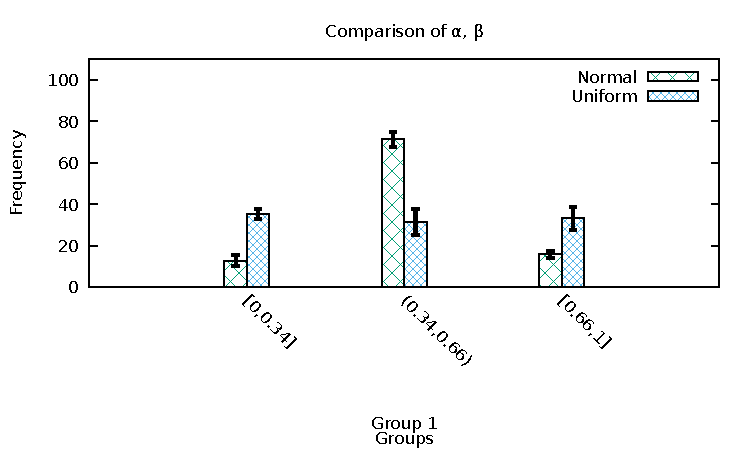
\includegraphics[scale=0.7]{graph1.pdf}
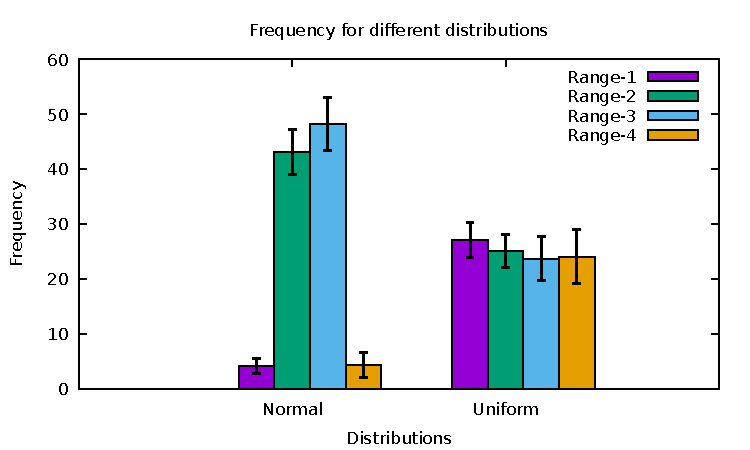
\includegraphics[scale=0.7]{graph2.pdf}
